\documentclass[10pt,aspectratio=43,mathserif]{beamer}
\usepackage{nju}			 %导入 nju 模板宏包
%\usepackage[UTF8]{ctex}      %导入 ctex 宏包,添加中文支持
\usepackage{xeCJK}
\usepackage{amsmath,amsfonts,amssymb,bm}   %导入数学公式所需宏包
\usepackage{color}			 %字体颜色支持
\usepackage{graphicx,hyperref,url}
\usepackage{listings}
\usepackage{booktabs}
\usepackage{multirow}
\usepackage{float}
\usepackage{mhchem}
\usepackage{animate}

\beamertemplateballitem		%设置 Beamer 主题
\catcode`\。=\active        %或者=13
\newcommand{。}{.}         %将正文中的“。”号转换为“.”。

%\AtBeginSection[]
%{
%  \begin{frame}
%    \frametitle{Contents}
%    \tableofcontents[currentsection]
%  \end{frame}
%}



\title{TS Investigation Exercise}	        %首页信息设置

\author[]{            %个人信息设置
    Shirong Wang\\[0.3cm]
    %15XXXXXXXX\\[0.3cm]
    Kuang Yaming Honors School}

\date{\today}



\begin{document}

\begin{frame}
\titlepage
\end{frame}

\begin{frame}
\frametitle{Contents}
\tableofcontents
\end{frame}

\section{$ S_N 2 $ of Chloromethane}
\begin{frame}
\frametitle{$ S_N 2 $ of Chloromethane}
\begin{equation}\label{key}
\ce{CH_3Cl + Br^- -> CH_3Br + Cl^-}
\end{equation}

\end{frame}


\begin{frame}
\begin{figure}
	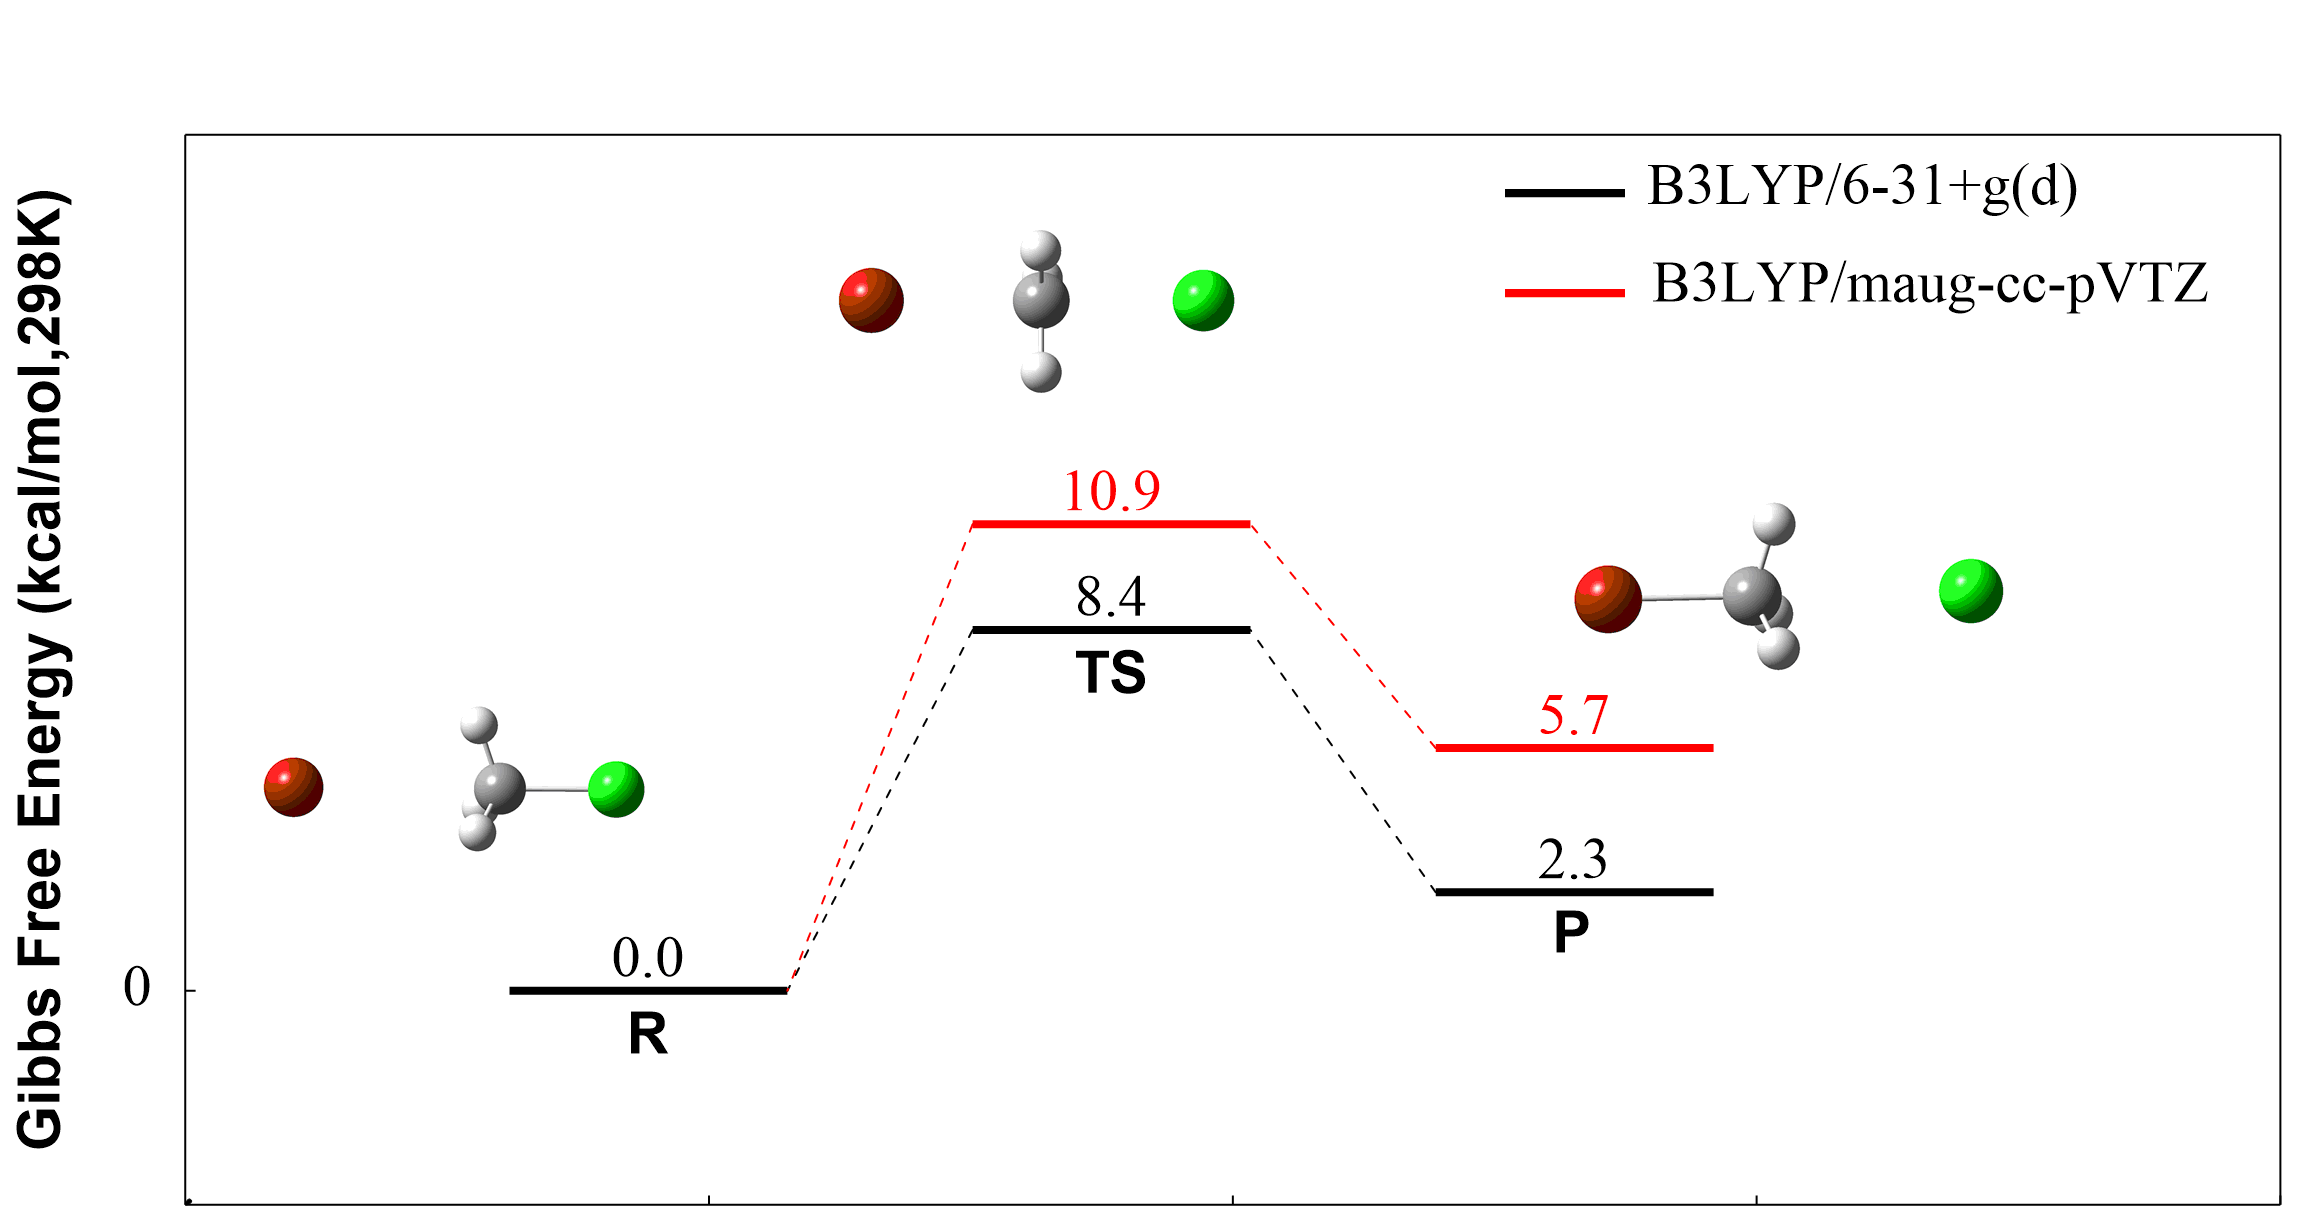
\includegraphics[width=\linewidth]{../sample/sn2c.png}
\end{figure}
\begin{table}[H]
	\begin{tabular}{ccccc}
		\hline
		& $ \ce{C-Cl} $ (R) & $ \ce{C-Cl} $ (TS) & $ \ce{C-Br} $ (TS) & $ \ce{C-Br} $ (P)\\ \hline
		B3LYP/6-31+g(d) & 1.856 & 2.370 & 2.482 & 2.021 \\
		B3LYP/maug-cc-pVTZ & 1.845 & 2.415 & 2.453 & 2.023 \\
		\hline
	\end{tabular}
    \caption{Bond length (\AA) in configurations above}
\end{table}
\end{frame}

\section{Claisen Rearrangement}
\begin{frame}
\frametitle{Claisen Rearrangement}
\begin{figure}[H]
	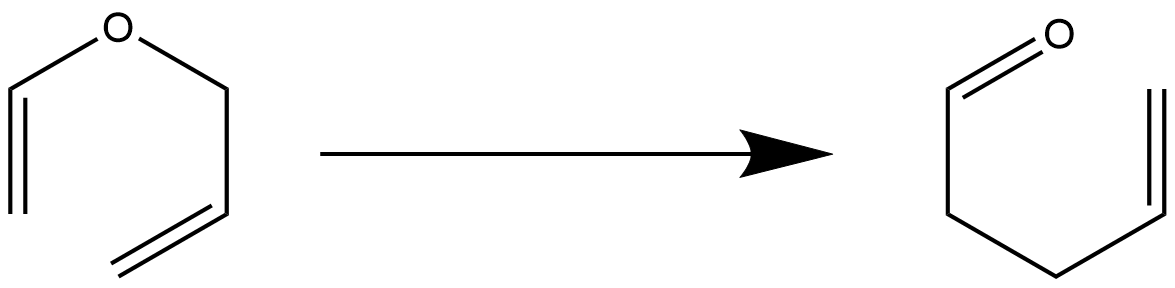
\includegraphics[width=0.6\linewidth]{claisen.png}
\end{figure}
\end{frame}

\begin{frame}
\frametitle{Transition State I -- Chair A}
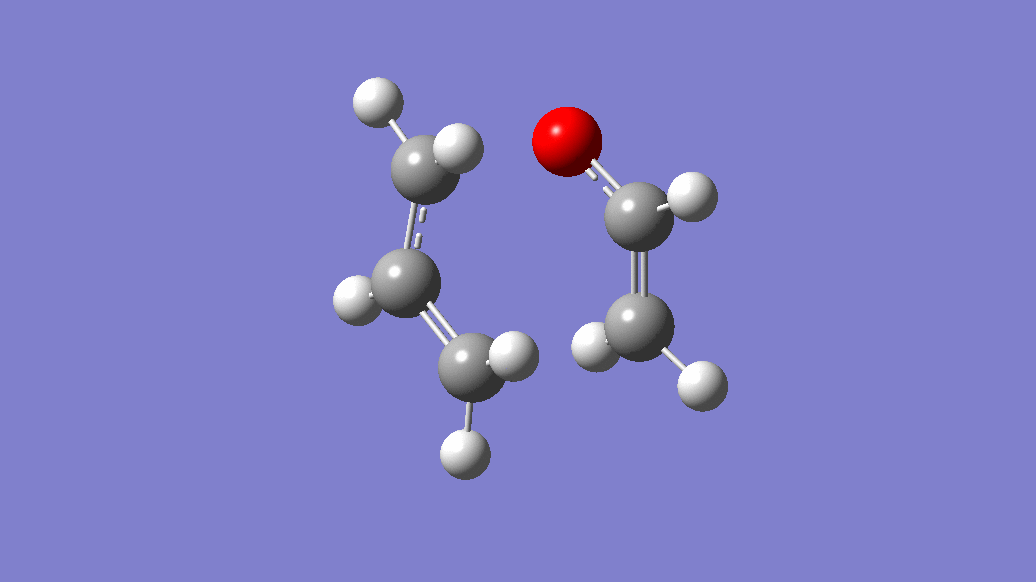
\includegraphics[width=0.4\linewidth]{../claisen/tsb4.png}
\animategraphics[width=0.4\linewidth,loop,controls]{20}{../claisen/tsb4_}{0}{48}
~\\
All the results in this case are calculated with B3LYP/6-31+g(d)
\end{frame}
\begin{frame}
\frametitle{Chair A}
\begin{figure}
	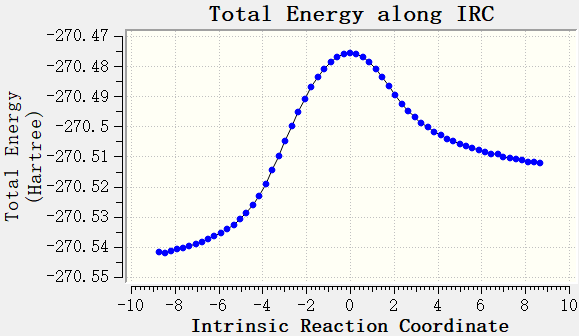
\includegraphics[width=0.8\linewidth]{../claisen/ircb4_tot_ener.png}
\end{figure}
\end{frame}

\begin{frame}
Extract the first and last structure from IRC and do optimization, we get the reactant and product
\begin{figure}
	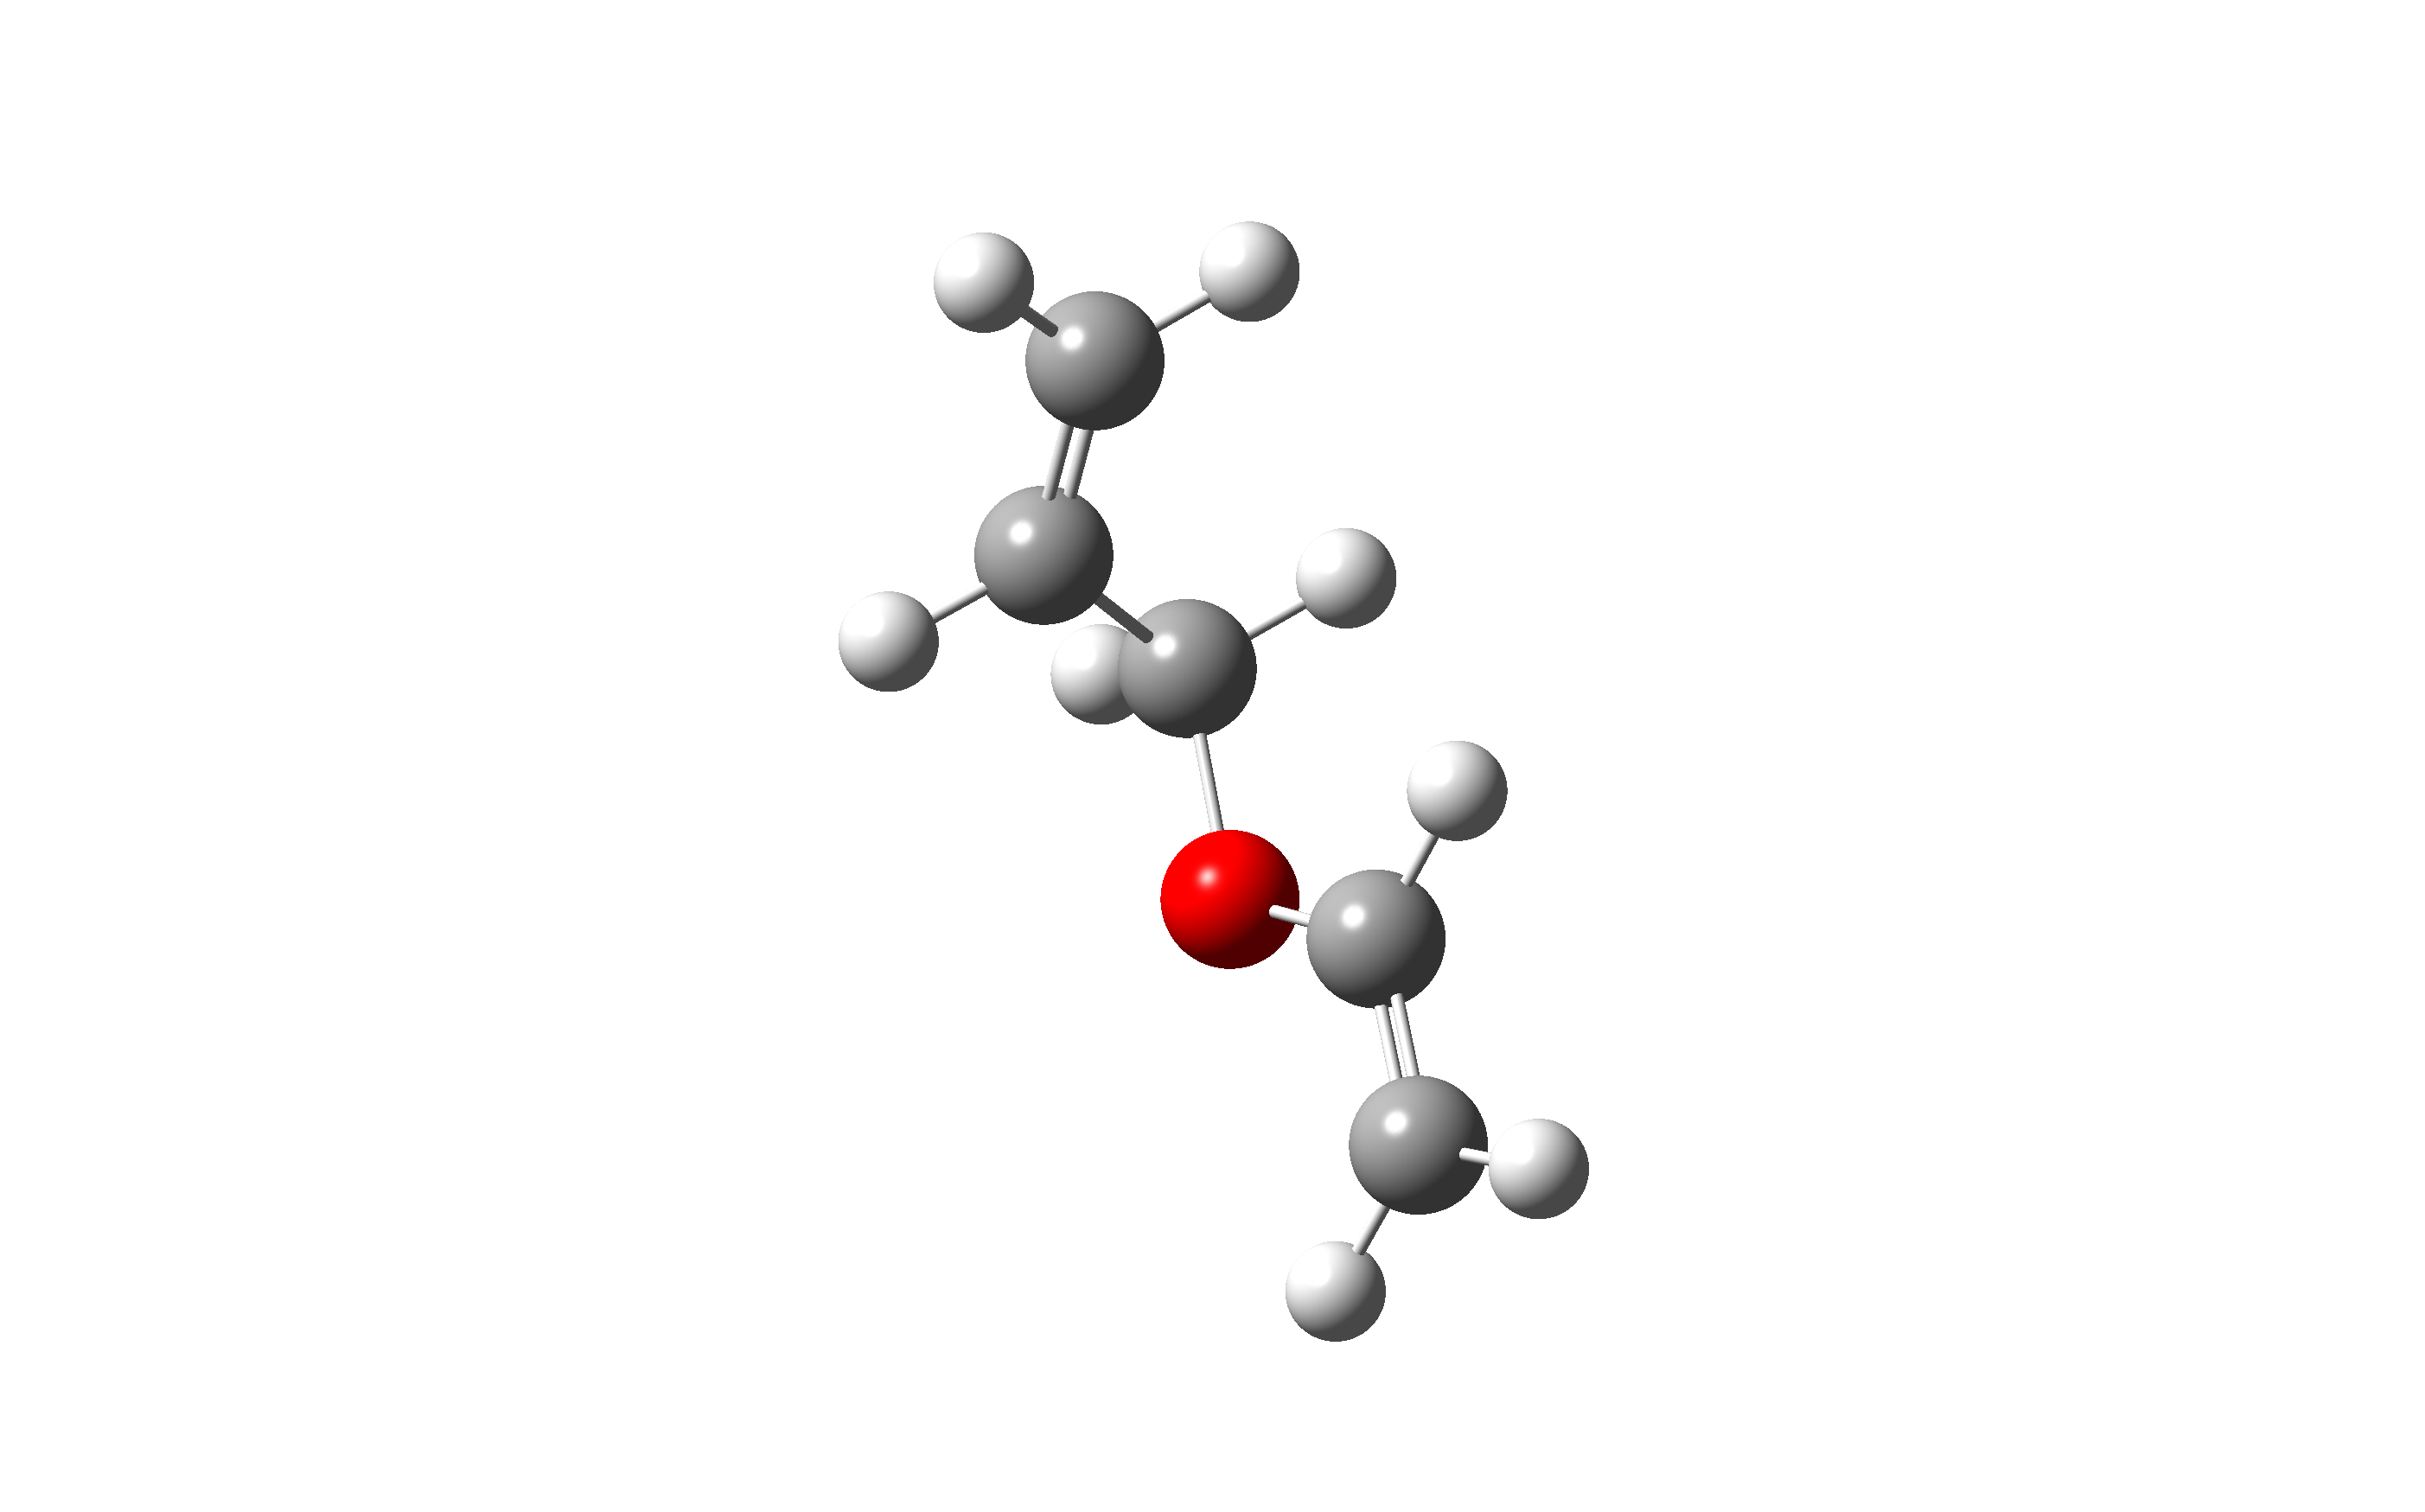
\includegraphics[width=0.45\linewidth]{../claisen/Rb4.png}
	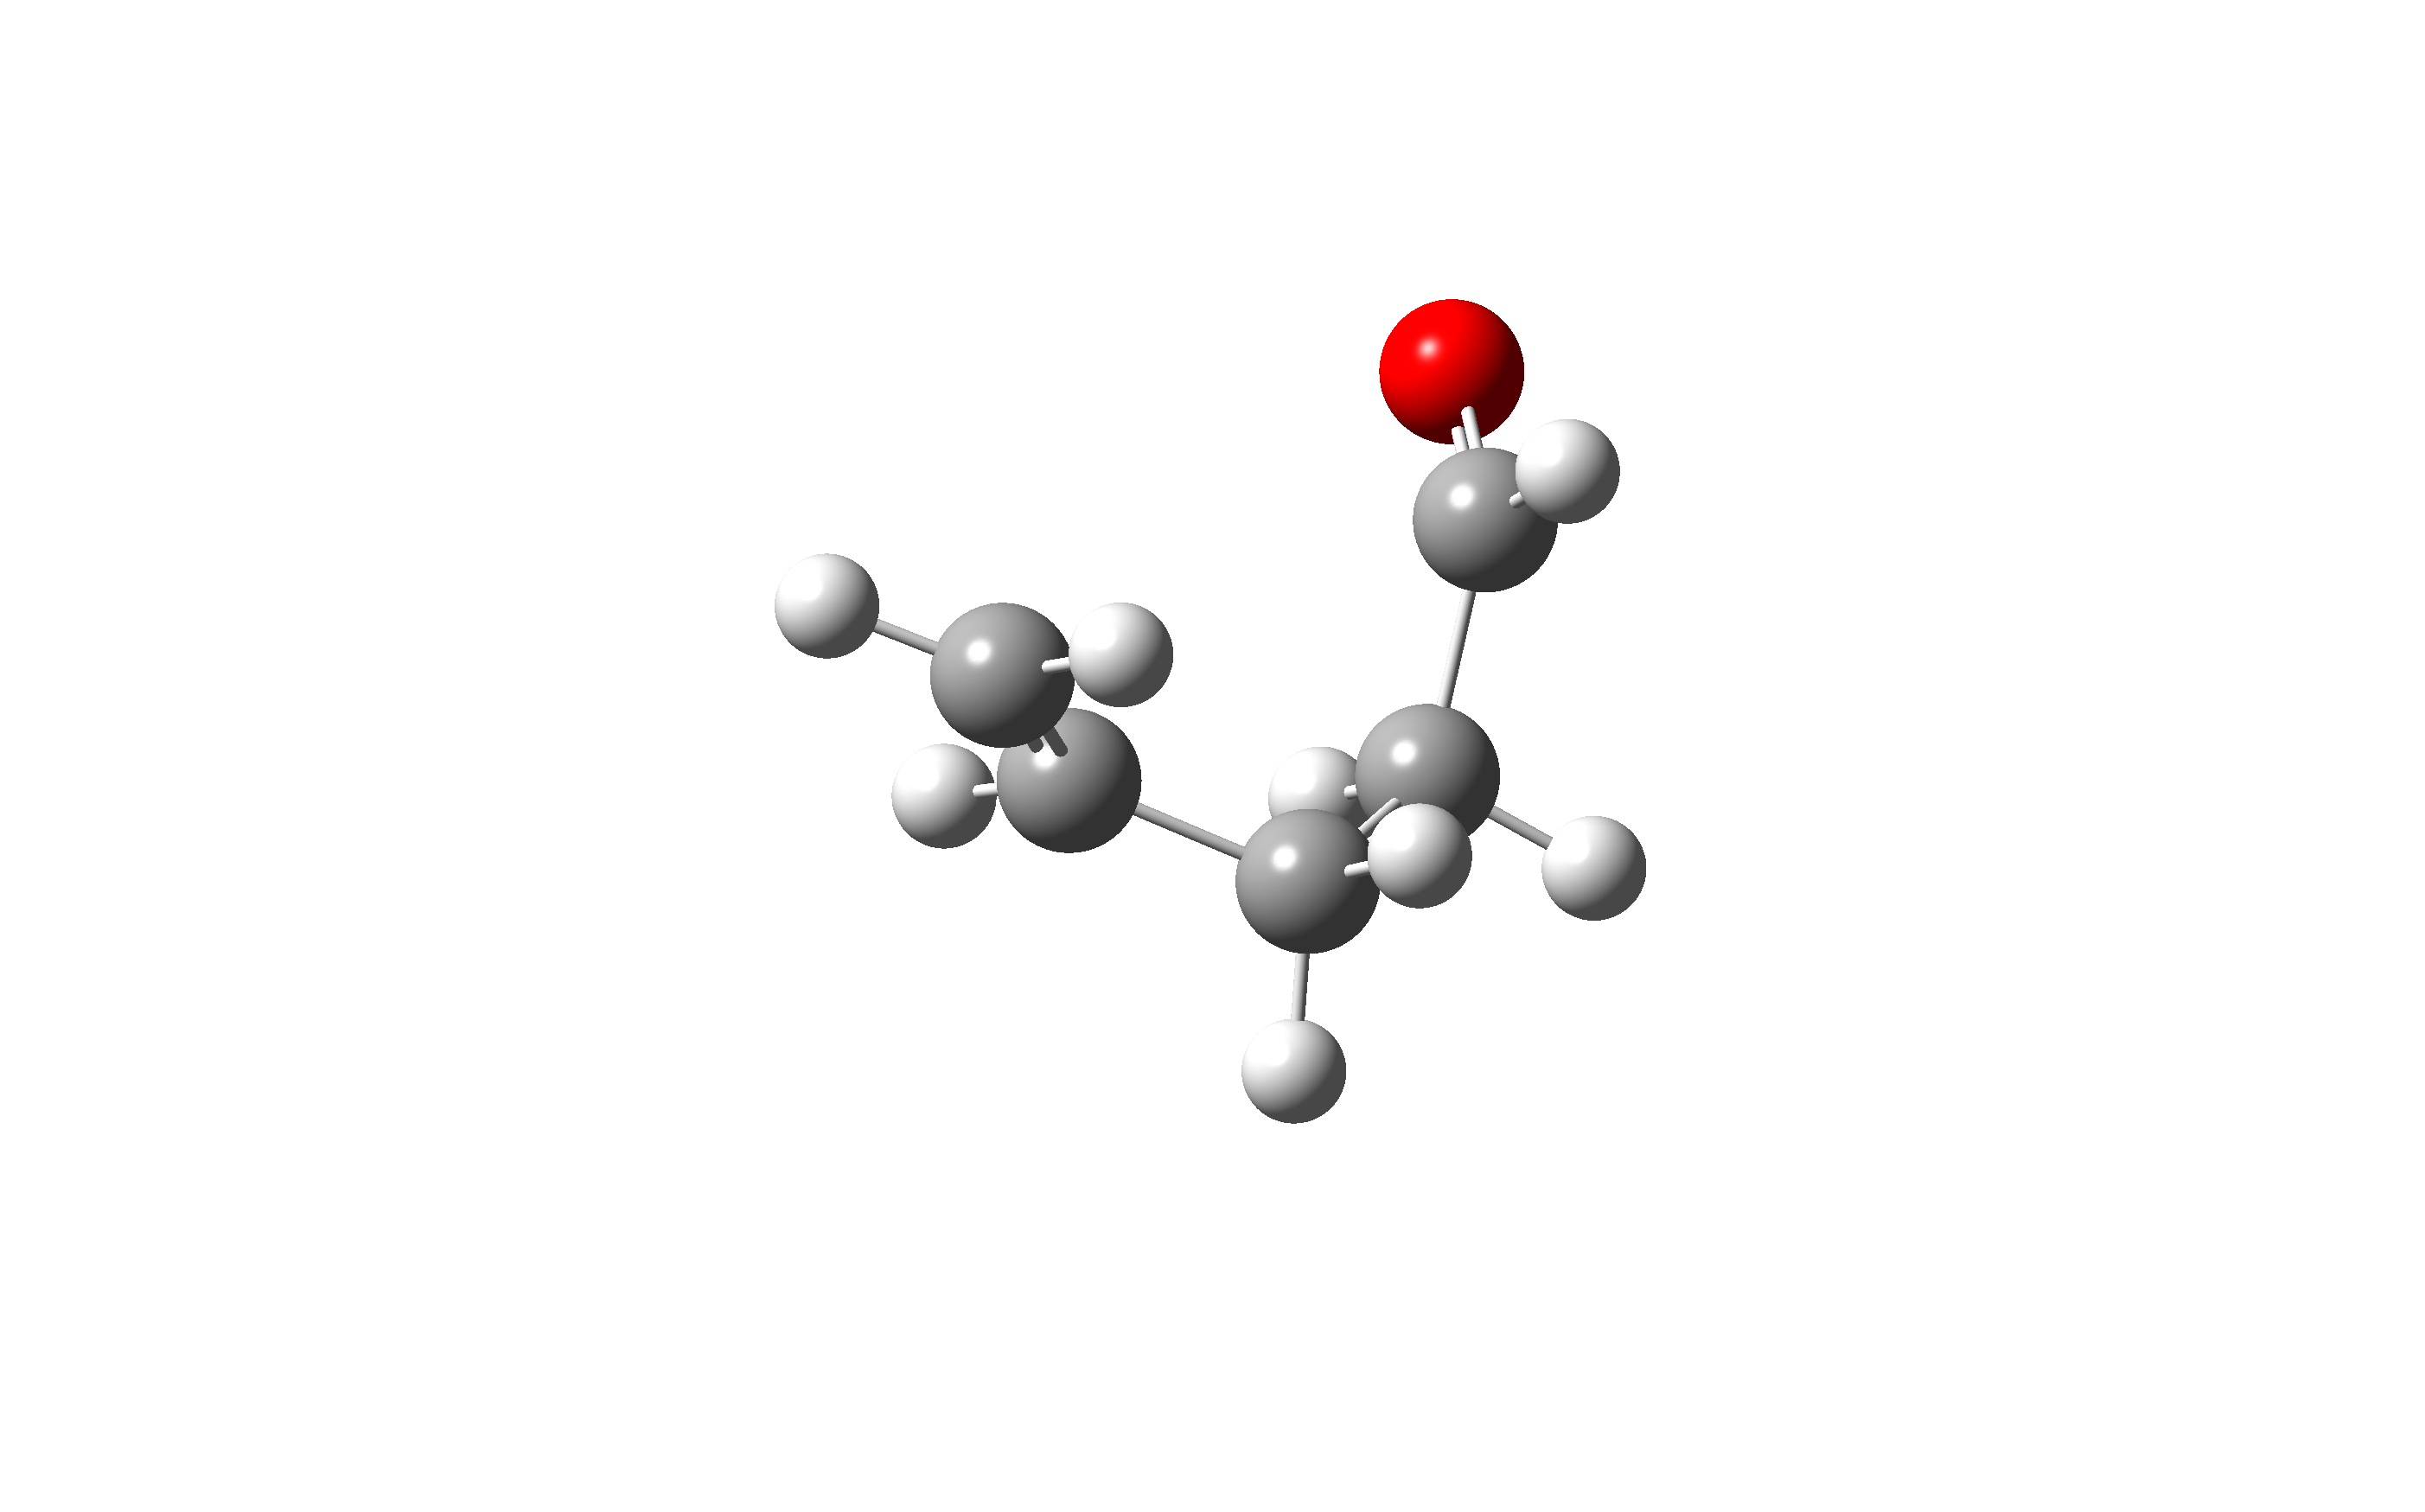
\includegraphics[width=0.45\linewidth]{../claisen/Pb4.png}
\end{figure}
\end{frame}

\begin{frame}
\begin{figure}
	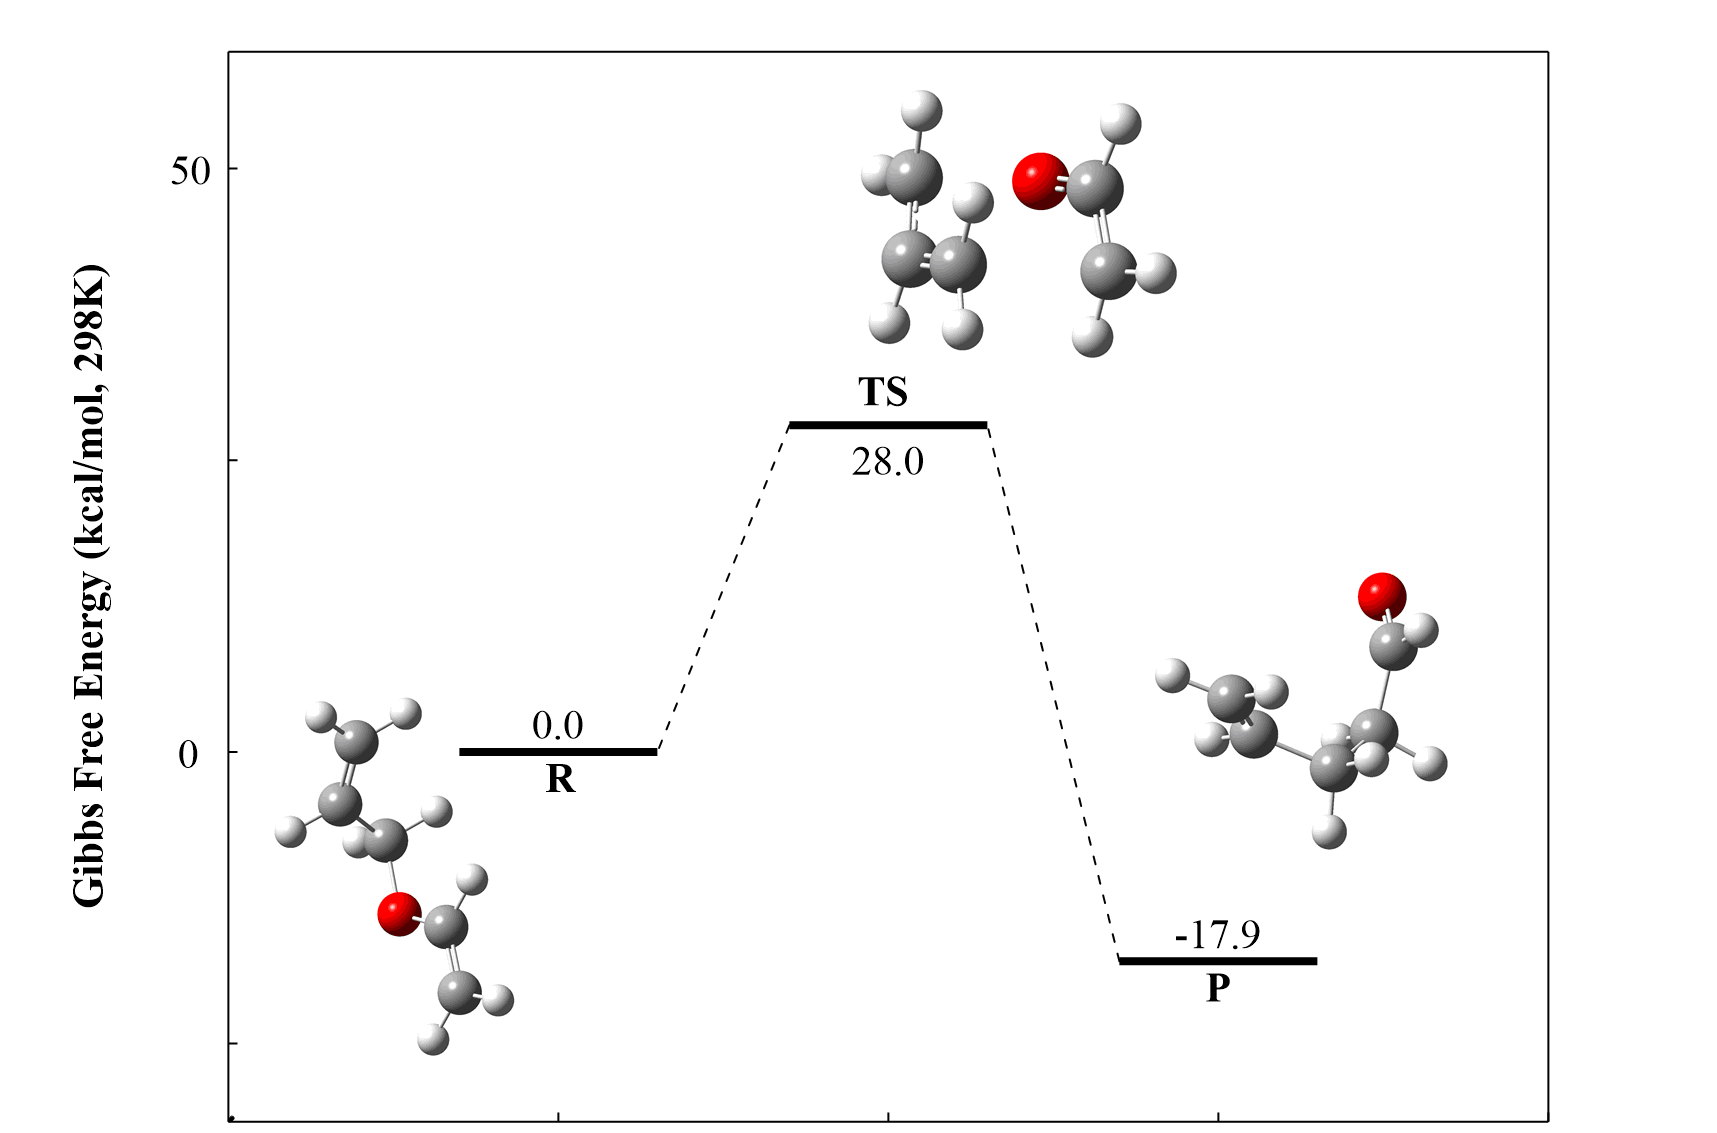
\includegraphics[width=0.8\linewidth]{../claisen/cl.png}
	%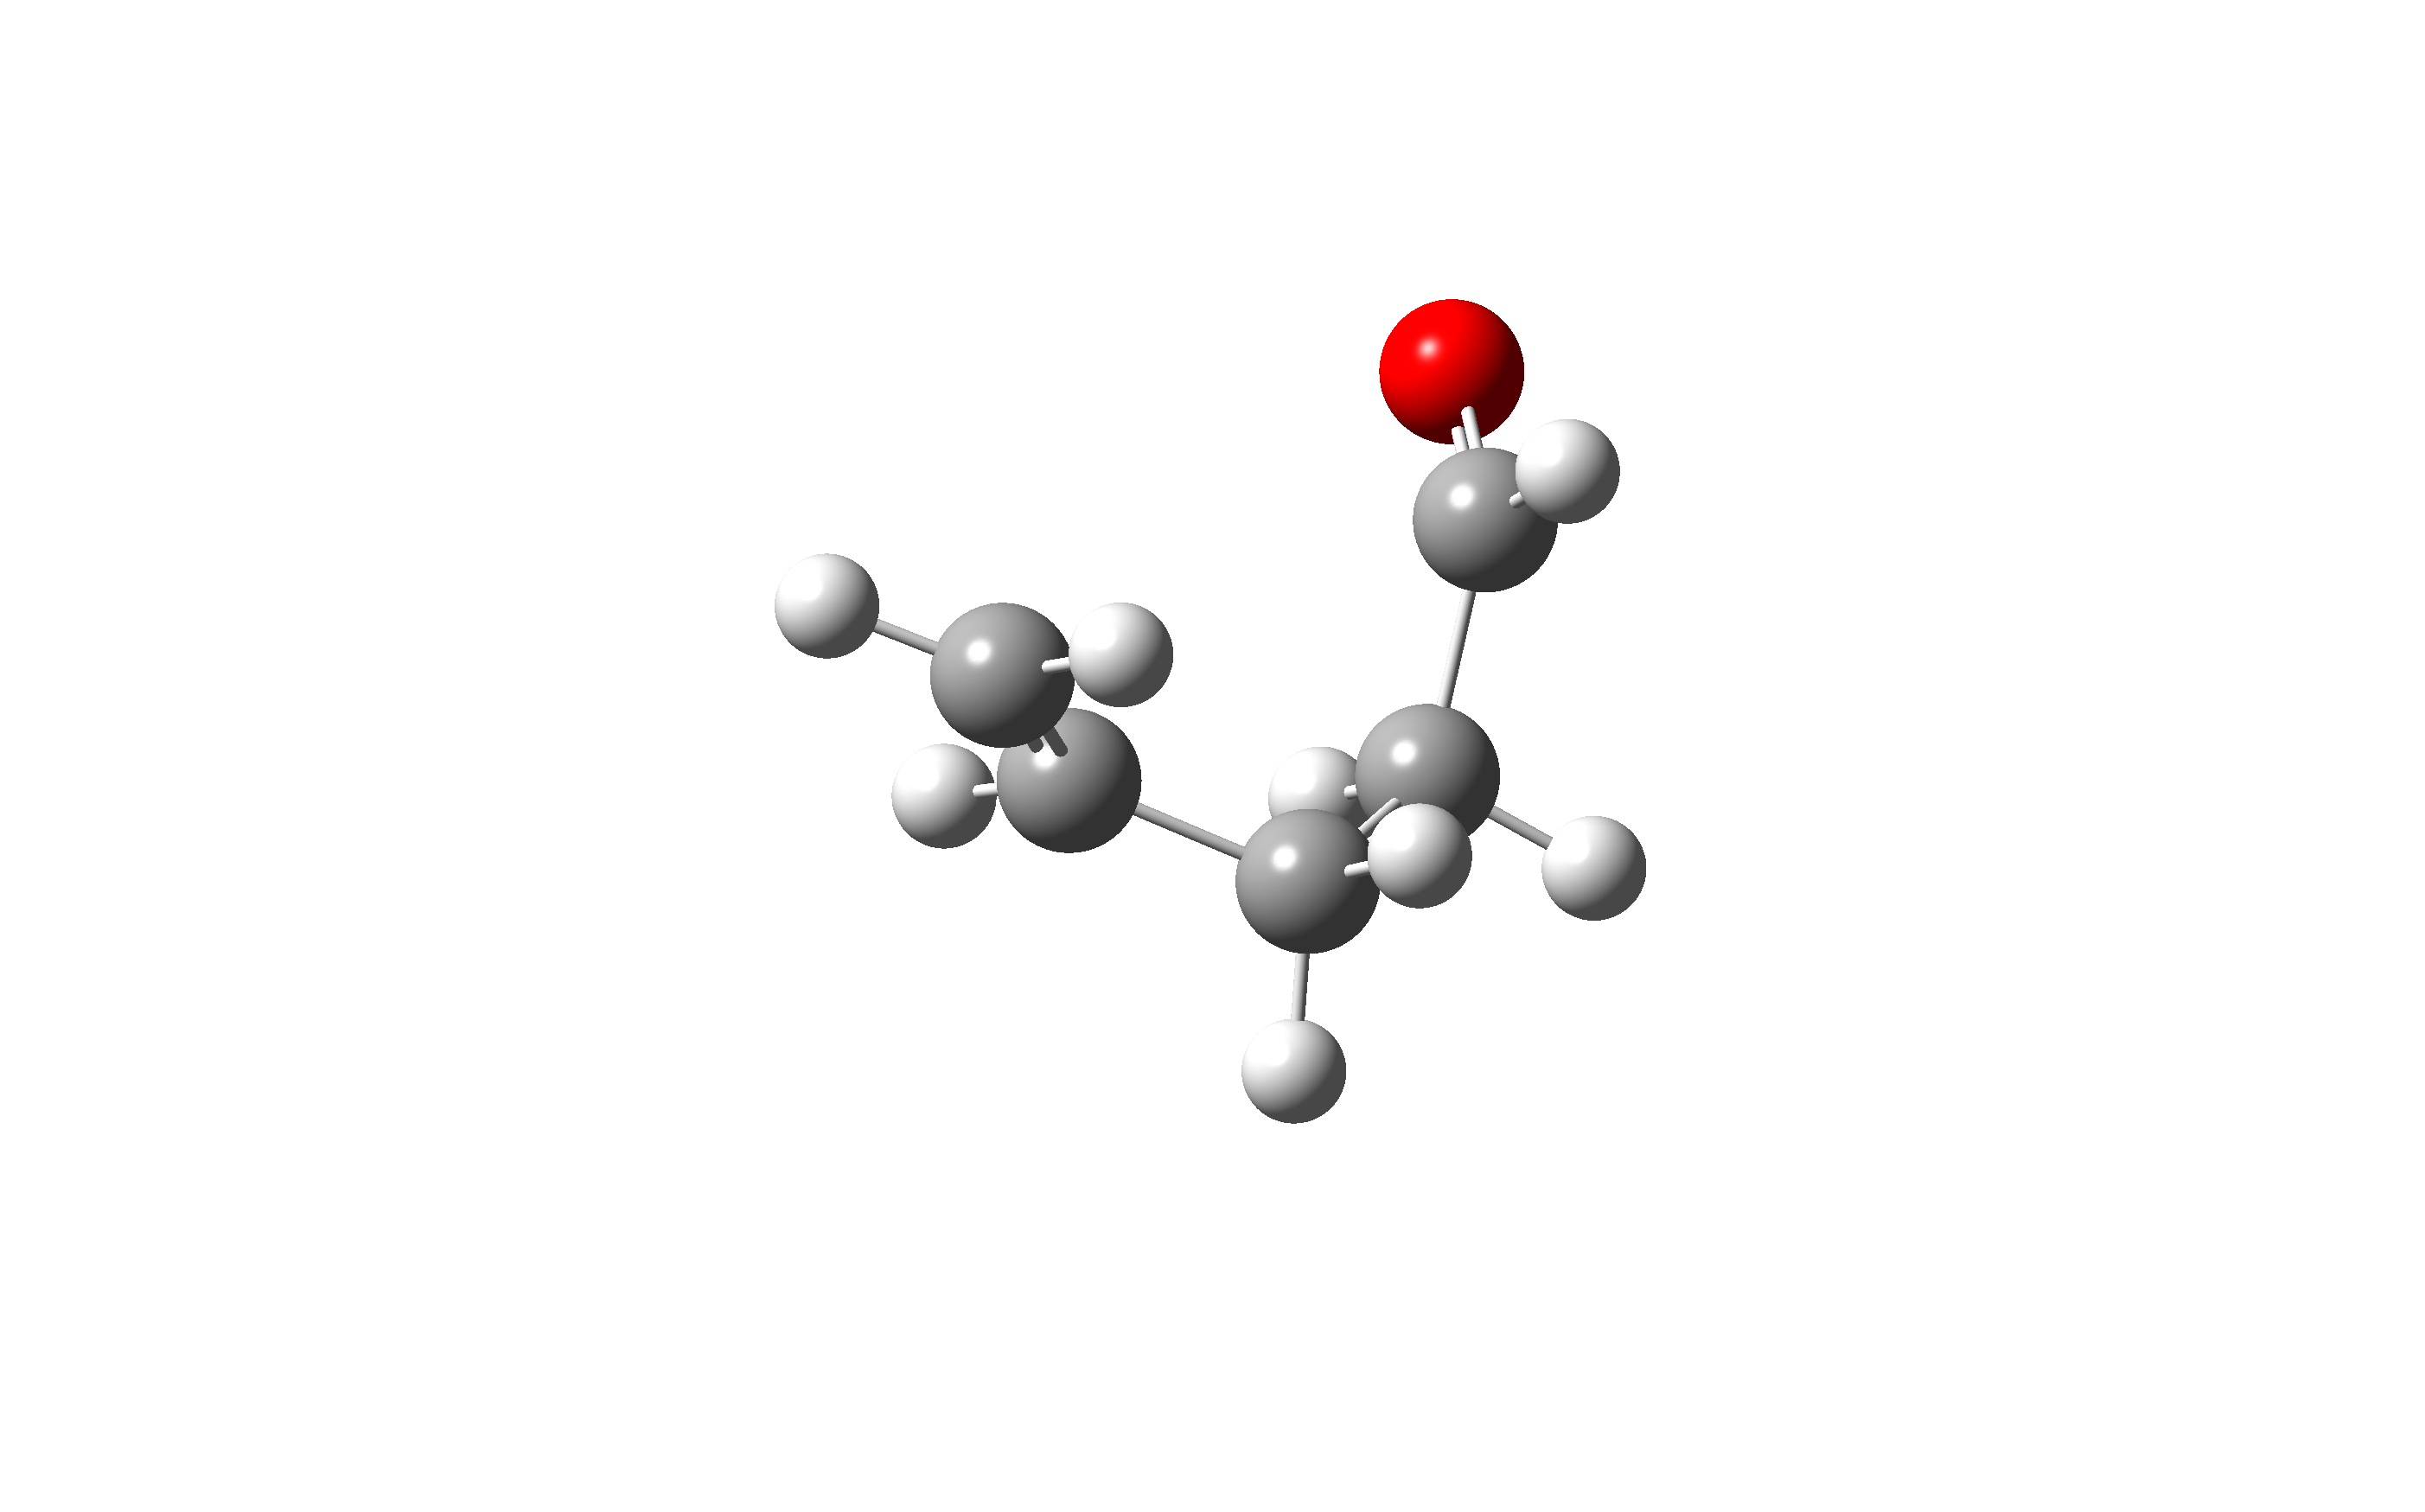
\includegraphics[width=0.45\linewidth]{../claisen/Pb4.png}
\end{figure}
\end{frame}

\begin{frame}
\frametitle{Transition State II -- Chair B}
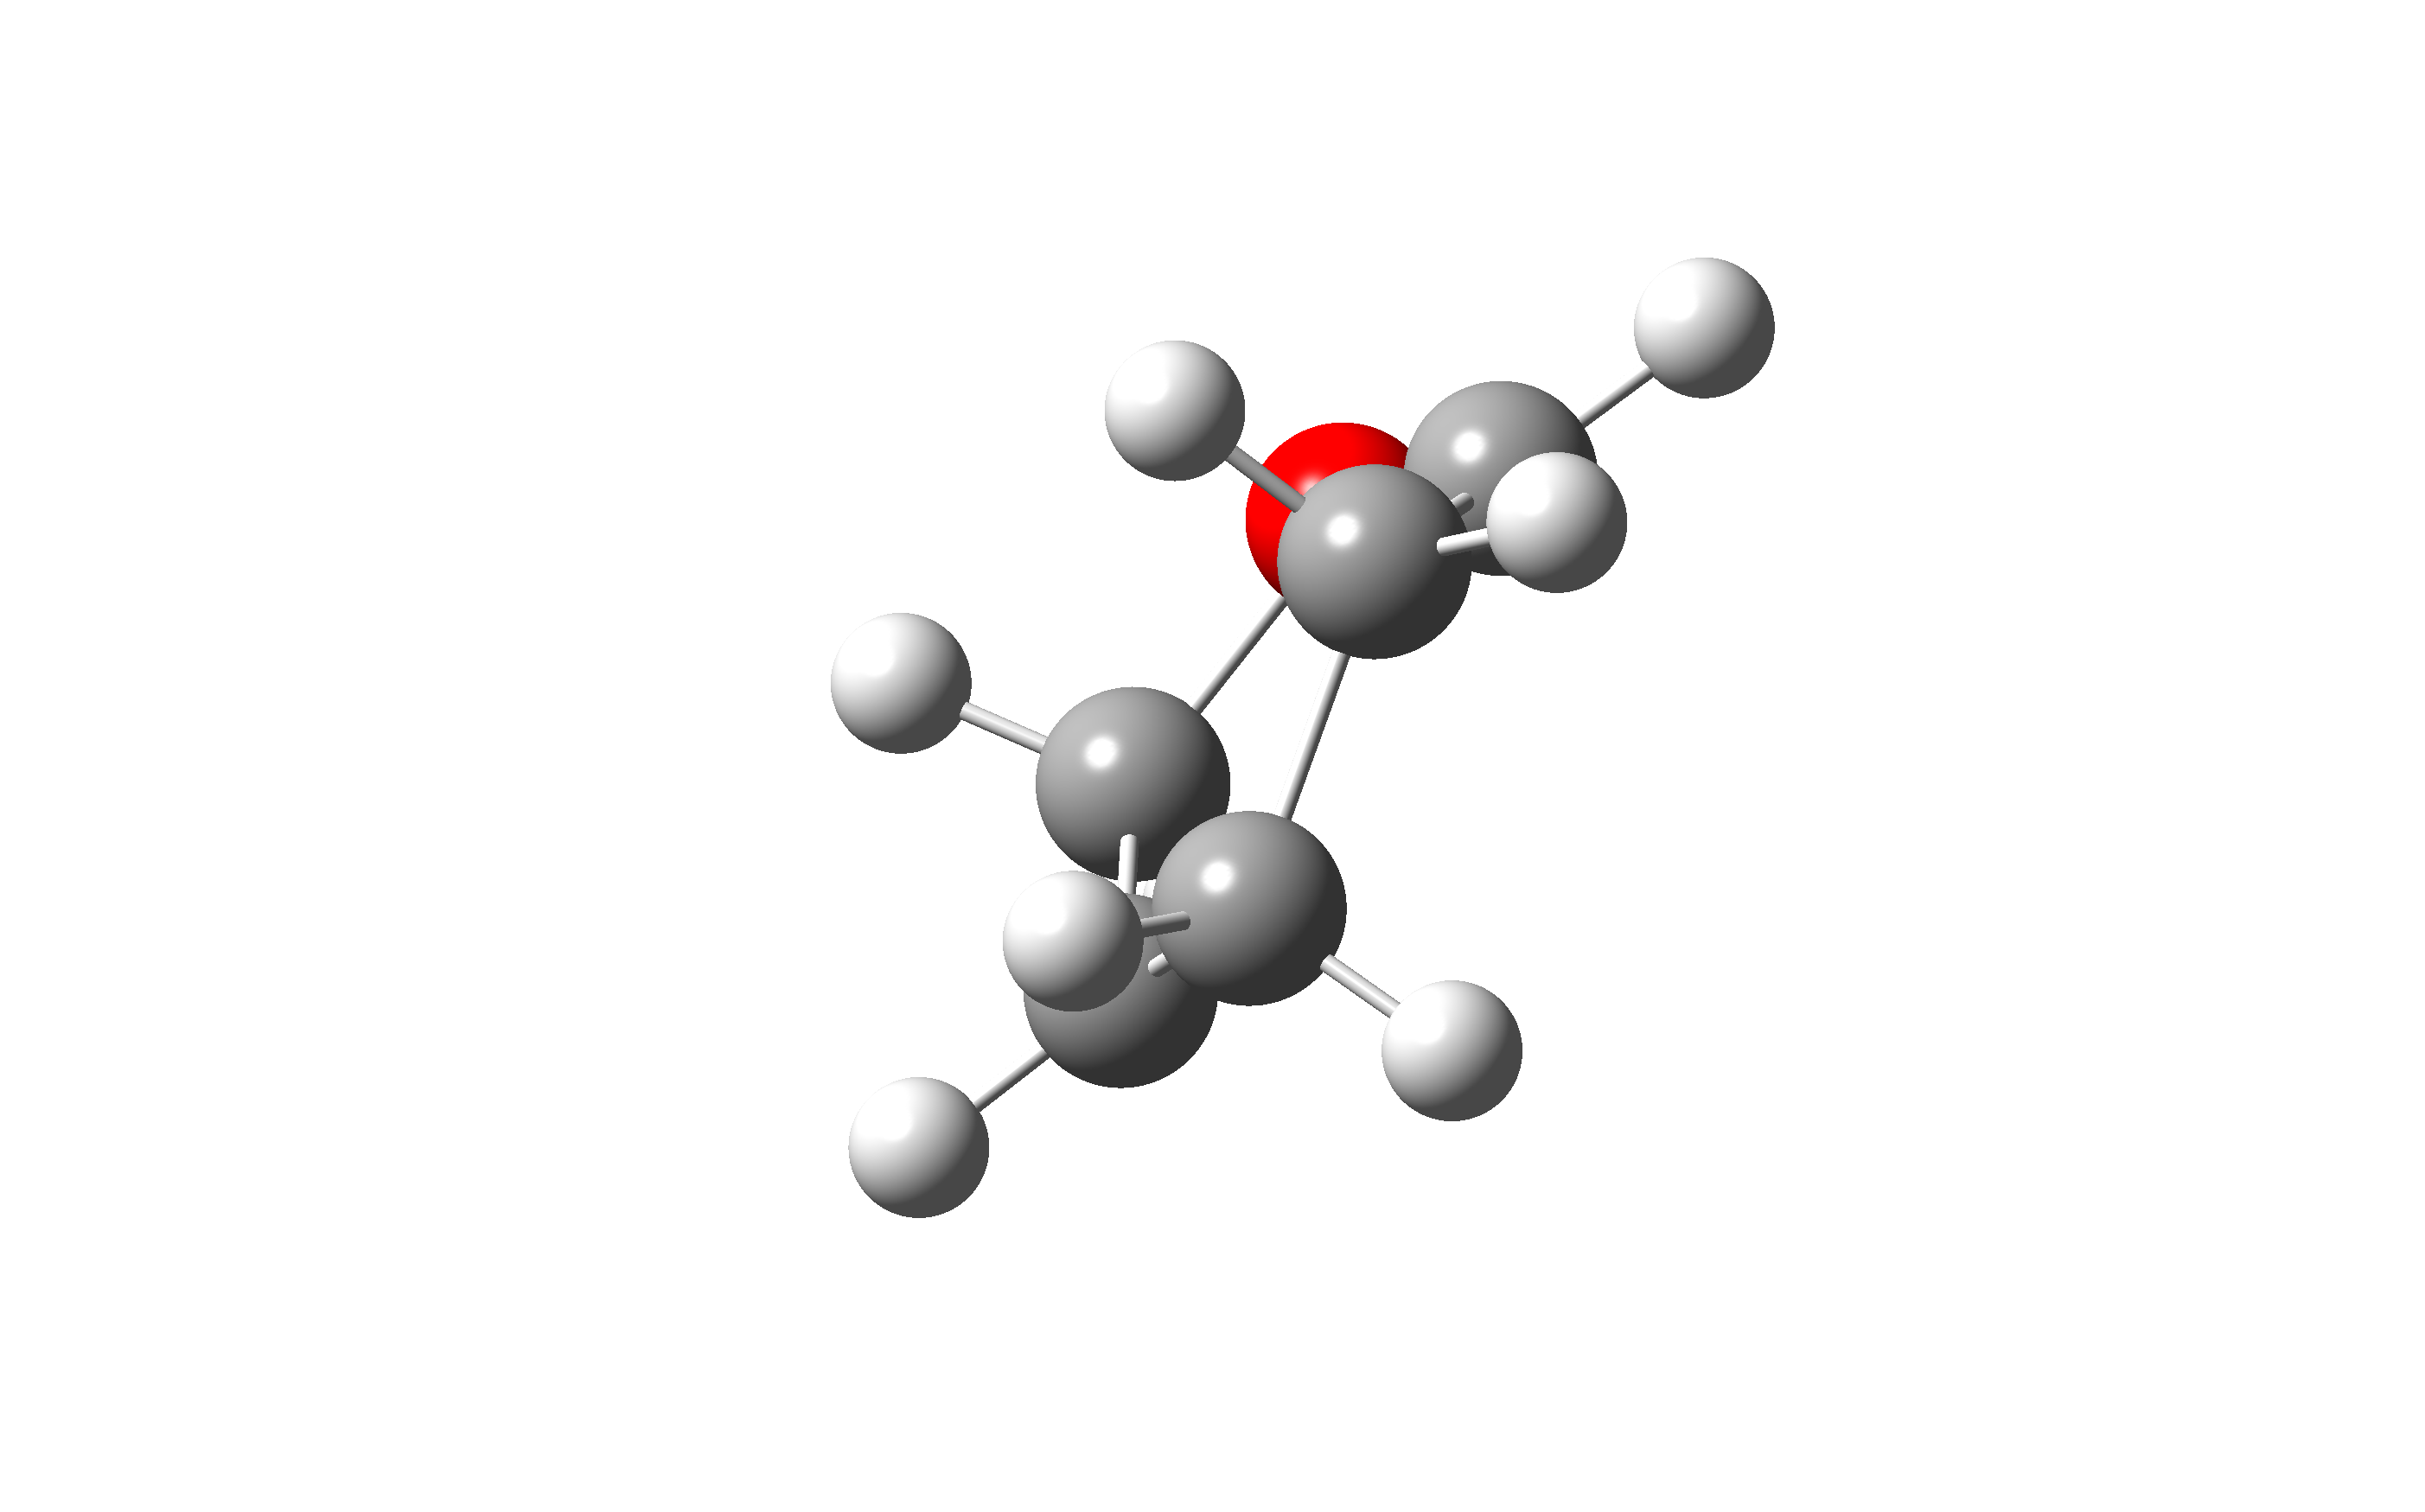
\includegraphics[width=0.4\linewidth]{../claisen/ts4.png}
%\animategraphics[width=0.4\linewidth,loop,controls]{20}{../claisen/tsb4_}{0}{48}
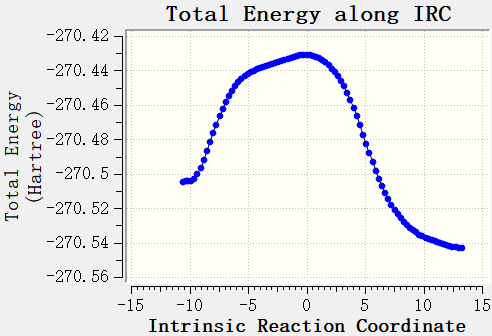
\includegraphics[width=0.5\linewidth]{../claisen/irc4_tot_ener.png}
\end{frame}

\begin{frame}
\frametitle{Others}
\begin{enumerate}
	\item Boat 
	\item ...
\end{enumerate}
\end{frame}


\section{Aldol Reaction}
\begin{frame}
\begin{equation}\label{key}
\ce{CH_2=CH-OH + O=CH_2 -> CHO-CH_2-CH_2-OH}
\end{equation}
\frametitle{Aldol Reaction}
\begin{figure}
	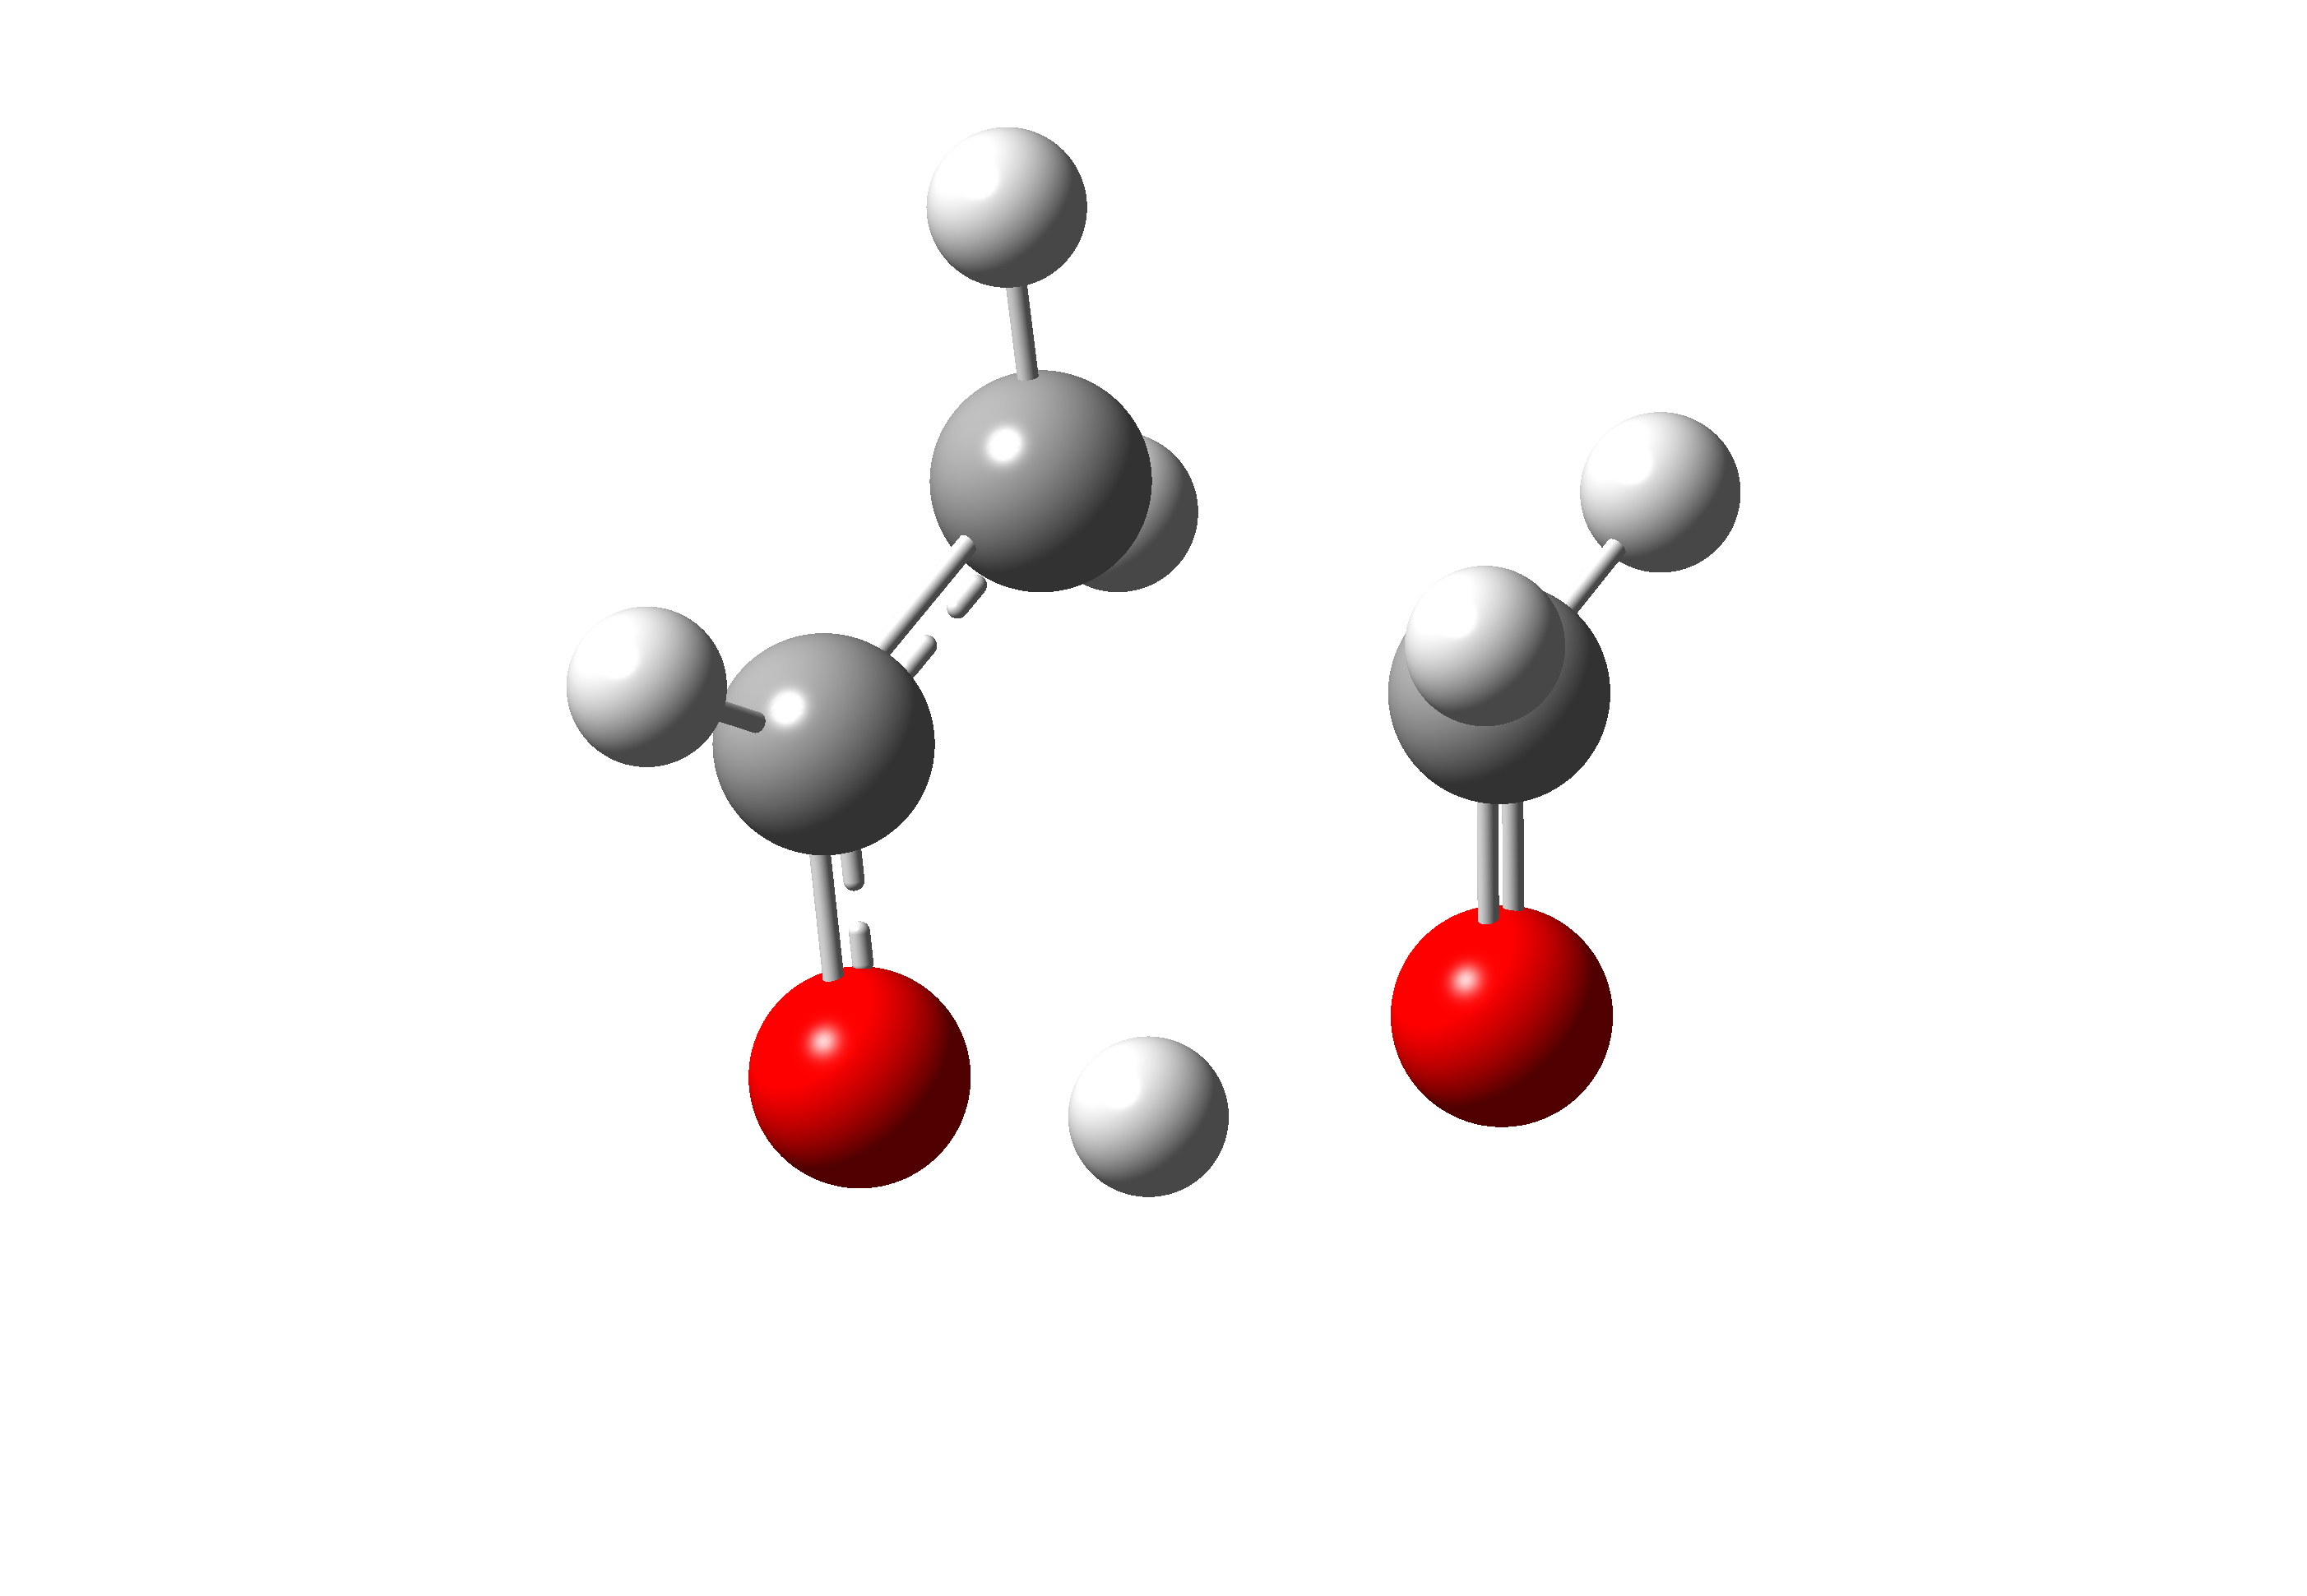
\includegraphics[width=0.4\linewidth]{../3/ts3.png}
	%\animategraphics[width=0.4\linewidth,loop,controls]{20}{../claisen/tsb4_}{0}{48}
	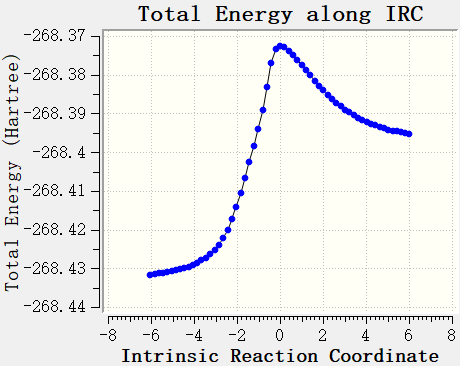
\includegraphics[width=0.5\linewidth]{../3/irc32_tot_ener.png}
\end{figure}
All calculated with B3LYP/6-311+g(d)
\end{frame}
\end{document}